\documentclass[11pt,a4paper]{article}

\usepackage{style2017}
\usepackage{hyperref}

\hypersetup{
    colorlinks =false,
    linkcolor=blue,
   linkbordercolor = 1 0 0
}
\newcounter{numexo}
\setcellgapes{1pt}

\begin{document}



\begin{NSI}
{TP}{Notation polonaise inverse}
\end{NSI}


\section{Étude théorique}

Nous allons étudier le fonctionnement d'une méthode de calcul appelée \textbf{notation polonaise inverse} utilisée par certaines calculatrices. La méthode permet de réaliser les calculs sans utiliser de parenthèses en respectant les priorités opératoires.

\subsection*{Description}

On appelle \textbf{opérande} un nombre entier ou décimal et \textbf{opérateur} une des quatre opérations parmi l'addition, la soustraction, la multiplication et la division.\medskip

On considère l'expression numérique $A=(8+3) \times 5$.\medskip

Elle se note en notation polonaise inverse par $8~3~+~5~\times$.\medskip

Sur une calculatrice, on tape sur la touche "Enter" entre les saisies de deux nombres.\medskip

\begin{itemize}
\item La notation polonaise inverse place les deux \textbf{opérandes} en premier et l'\textbf{opérateur} après (et non au centre), donc l'addition $8+3$ se note $8~3~+$;
\item Les priorités opératoires déterminent l'ordre de la notation permettant de supprimer les parenthèses. L'expression $8~3~+~5~\times$ indique que l'on commence par l'addition avant la multiplication nécessitant des parenthèses dans l'écriture classique.
\end{itemize}

Les opérandes et les résultats des différentes opérations sont enregistrés dans une pile. Lorsque le calcul se termine, la pile ne contient plus que le résultat de l'expression calculée. 

\subsection*{Quelques cas pratiques}
\begin{enumerate}
\item Donner la notation polonaise inverse des expressions numériques suivantes:
\begin{enumerate}
\item $8 \times (7-4)$
\item $(9-5)(7+2)$
\item $4 \times 3 \times 2 \times 1$
\item $15-4\times 7 + 9$
\end{enumerate}
\item Calculer les expressions suivantes:
\begin{enumerate}
\item $7~6~+~2~/$
\item $5~3~*~2~7~*~-$
\end{enumerate}
\item Pour calculer en notation polonaise inverse, on utilise une pile qui stocke les valeurs numériques au fil des opérations. On donne les différents états de la pile de calcul de l'exemple initial:
\begin{center}
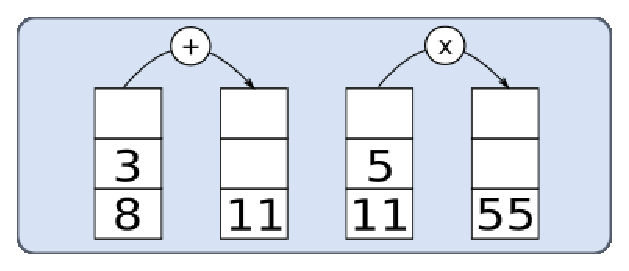
\includegraphics[scale=0.6]{../../img/exNotPolInv1.eps}
\end{center}
\begin{enumerate}
\item Représenter les états de la pile de l'expression \textbf{2)~a)}.
\item Comment se déroule l'empilement et le dépilement de la pile dans un calcul ?
\end{enumerate}

\end{enumerate}


\section{Programmation en python}

On utilise l'implémentation des piles créées avec les listes lors des exercices précédents. On s'assure de bien avoir les fonctions suivantes:
\begin{itemize}
\item cree\_pile() qui crée une pile vide;
\item empile(v, p) qui ajoute la valeur v au sommet de la pile p;
\item depile(p) qui récupère le sommet de la pile p en le supprimant;
\item pile\_vide() qui teste si la pile est vide (booléen).
\end{itemize}\medskip

Chaque expression numérique est enregistrée dans une liste:
\begin{itemize}
\item les opérandes sont enregistrés en tant que nombres : type \textbf{int} ou \textbf{float};
\item les opérateurs sont enregistrés comme chaine de caractères : type \textbf{string}.
\end{itemize}\medskip

Par exemple, l'expression $8~3~+~5~\times$ est enregistrée dans la liste $[8,~3,"+",~5,~"*"]$.\medskip

Voici l'algorithme qui permet de calculer une expression en notation polonaise inverse:\medskip

\begin{center}
\begin{tabular}{|p{10cm}|}
\hline
Pour $e$ dans expression:\\
\hspace{1cm}si $e$ est un nombre:\\
\hspace{2cm}on empile le nombre\\
\hspace{1cm}sinon:\\
\hspace{2cm}on dépile 2 opérandes\\
\hspace{2cm}on effectue l'opération\\
\hspace{2cm}on empile le résultat\\
on renvoie le résultat\\
\hline
\end{tabular}
\end{center}



\begin{enumerate}
\item Écrire une fonction \textbf{operation} qui prend en paramètres 2 nombres \textbf{a} et \textbf{b} et un opérateur \textbf{op} et renvoie le résultat de l'opération \textbf{a op b}. Il faudra traiter les quatre opérations dans la même fonction.
\item Écrire une fonction \textbf{calcule} qui prend en paramètre l'expression à calculée sous forme de liste et renvoie le résultat.
\item Tester votre programme avec les opérations de la première partie.
\end{enumerate}


%\section{Pour aller plus loin}
%Cette partie est facultative mais permet d'approfondir la réflexion. Les questions sont indépendantes.
%\begin{enumerate}
%\item Créer une fonction qui prend en saisie, au clavier, une expression en notation polonaise inverse et la renvoie sous forme de liste en respectant le type des valeurs saisies.
%\item Créer une fonction qui prend en saisie une expression en notation classique avec au plus 2 opérations et la transforme en notation polonaise inverse.
%\end{enumerate}

\end{document}
